\documentclass[handout]{beamer}
% 2 Standard packages f�r die deutsche Sprache
\usepackage[ngerman]{babel}
\usepackage[latin1]{inputenc}
\usepackage[markup=nocolor]{changes}
\usepackage{color}
\title[Crisis] % (optional, only for long titles)
{Botnetze und Trojaner}
%\subtitle{und Trojaner}
\author{M.~Pfuhl}
\date{IT-Sicherheit, Juni 2016}
\subject{Computer Science}
\beamertemplatenavigationsymbolsempty
\setbeamertemplate{footline}[text line]{%
  \parbox{\linewidth}{\vspace*{-8pt}Botnetze und Trojaner\hfill\insertshortauthor\hfill\insertframenumber/\inserttotalframenumber}}
\begin{document}

	{
		\setbeamertemplate{footline}{}
		\frame{\titlepage}
		
		\frame{
			\frametitle{Inhaltsangabe}
			\tableofcontents
		}
	}
	
	\addtocounter{framenumber}{-2}
	
	\section{Motivation}
  \frame{
    \frametitle{Motivation}
		\begin{itemize}[<+->]
			\item Bagle (2004)
			\begin{itemize}
				\item immer noch aktiv
				\item urspr�nglich Wurm
			\end{itemize}
			\item Storm (2004)
			\begin{itemize}
				\item immer noch aktiv
			\end{itemize}
			\item Mariposa (2008)
			\begin{itemize}
				\item Dezember 2009 zerschlagen
				\item 12 Millionen Bots - kontrolliert von 3 Admins
			\end{itemize}
			\item Conficker (2008)
			\begin{itemize}
				\item immer noch aktiv
				\item Verbreitung und Versionierung
			\end{itemize}
			\item BredoLab (2009)
			\begin{itemize}
				\item November 2010 zerschlagen (nicht komplett)
				\item 30 Millionen Bots
			\end{itemize}
		\end{itemize}
  }
	
	\frame{
    \frametitle{Motivation}
		\begin{tabular}{|c|c|c|c|c|}
			\hline
			\textbf{Name}  & \textbf{entdeckt} & \textbf{zerschlagen} & \textbf{\#Bots} & \textbf{Spam/Tag}\\\hline
			Bagle & 2004 & - & 230.000 & 5,7 Mrd\\\hline
			Storm & 2004 & - & 160.000 & 3 Mrd\\\hline
			Mariposa & 2008 & 2009 & 12 Mio & -\\\hline
			Conficker & 2008 & - & 10,5 Mio & 10 Mrd\\\hline
			BredoLab & 2009 & \textit{2010} & 30 Mio & 6 Mrd\\\hline
		\end{tabular}
  }
	
	\section{Botnetz}
	\subsection{Begriffe}
	\frame{
		\frametitle{Botnetz}
		\framesubtitle{Begriffe}
		\pause
		\begin{itemize}[<+->]
			\item Bot (Zombie) - \textit{Opfer}
			\item Bot-Operator (-Herder, -Master) - \textit{Command\&Control}
		\end{itemize}
	}
	
	\subsection{Aufbau}
	\frame{
		\frametitle{Botnetz}
		\framesubtitle{Aufbau}
		\begin{itemize}[<+->]
			\item Client-Server Modell\\\vspace{\baselineskip}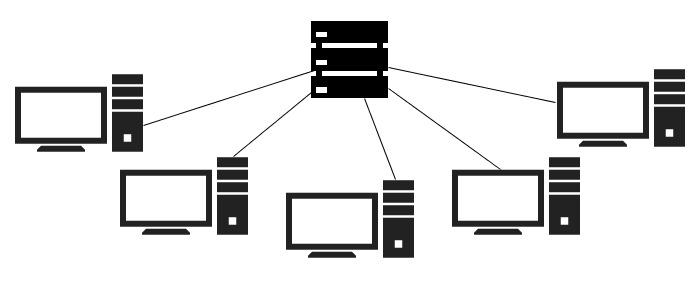
\includegraphics[scale=0.2]{client-server.png}
			\item Peer-to-Peer Modell\\\vspace{\baselineskip}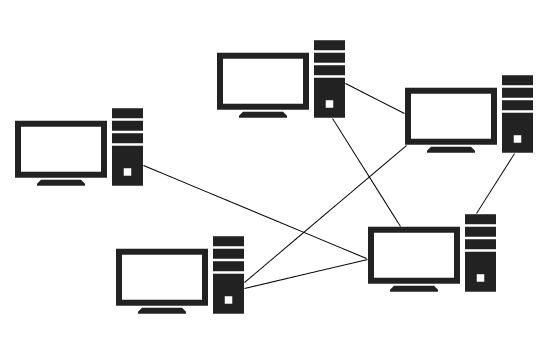
\includegraphics[scale=0.2]{peer-to-peer.png}
		\end{itemize}
	}
	
	\subsection{Command \& Control}
	\frame{
		\frametitle{Botnetz}
		\framesubtitle{Command \& Control}
		\begin{itemize}[<+->]
			\item IRC
			\item DNS
			\item webbasiert
			\begin{itemize}
				\item Port 80
				\item \textit{Push} statt \textit{Pull}
				\item Skalierbarkeit und Benutzbarkeit
				\item Echo-based
				\item Command-based
			\end{itemize}
			\item Peer-to-Peer
			\item FTP
		\end{itemize}
	}
	
	\subsection{Verbreitung}
	\frame{
		\frametitle{Botnetz}
		\framesubtitle{Verbreitung}
		\begin{itemize}[<+->]
			\item Malware (E-Mails)
			\item Downloads (Trojaner)
			\item Exploits
			\item Manuelle Installation
		\end{itemize}
	}
	
	\subsection{Anwendung}
	\frame{
		\frametitle{Botnetz}
		\framesubtitle{Anwendung}
		\begin{itemize}[<+->]
			\item legal
			\begin{itemize}
				\item Distributed Computing
			\end{itemize}
			\item illegal
			\begin{itemize}[<+->]
				\item Bot-extern
				\begin{itemize}[<+->]
					\item DDoS
					\item Proxy
					\item Click Fraud
					\item Spam Mails
				\end{itemize}
				\item Bot-intern
				\begin{itemize}[<+->]
					\item Sniffing
					\item Ransomware
					\item Filesharing
					\item Rechenleistung (Bitcoin)
				\end{itemize}
			\end{itemize}
			
		\end{itemize}
	}
	
	\section{Analyse Storm}
	\frame{
		\frametitle{Analyse \textit{Storm}}
		\begin{itemize}[<+->]
			\item Client-Server
			\item Peer-to-Peer
		\end{itemize}
	}
	
	\section{BYOB}
	\frame{
		\frametitle{BYOB}
		\begin{itemize}[<+->]
			\item \deleted{Bring Your Own Beer}\\Build Your Own Botnet
			\item \texttt{tentoB}\\
\includegraphics[scale=0.2]{tentob.png}
			\item \url{https://github.com/Sonnywhite/tentob}
		\end{itemize}
		
	}
	
	\frame{
		\frametitle{Build Your Own Botnet - \texttt{tentoB}}
		\framesubtitle{Infrastruktur}
		\begin{itemize}[<+->]
			\item 3 Clients (Bots)\\
				\texttt{Java}
			\item 1 Server (Bot-Operator)\\
				\texttt{Apache2, PHP, JavaScript, MySQL}
			\item \texttt{HTTP} als Kommunikationskanal
			\item \textit{Pull} statt \textit{Push}
			\item Echo-based
			\item Command-based
		\end{itemize}
	}
	
	\frame{
		\frametitle{Build Your Own Botnet - \texttt{tentoB}}
		\framesubtitle{Features}
		\begin{itemize}[<+->]
			\item Server-Seite
			\begin{itemize}
				\item Darstellung der einmaligen neuen Zugriffe\\(Nachweis des Angriffs)
				\item �berlick �ber Bots
				\item Ausl�sen von Attacken
			\end{itemize}
			\item Client-Seite
			\begin{itemize}
				\item Verbindung zum C\&C-Server mit Bot-ID (MAC-Adresse)
				\item Durchf�hrung einer DDoS-Attacke
			\end{itemize}
		\end{itemize}
	}
	
	\frame{
		\frametitle{Build Your Own Botnet - \texttt{tentoB}}
		\framesubtitle{Ablauf Client-Anwendung}
		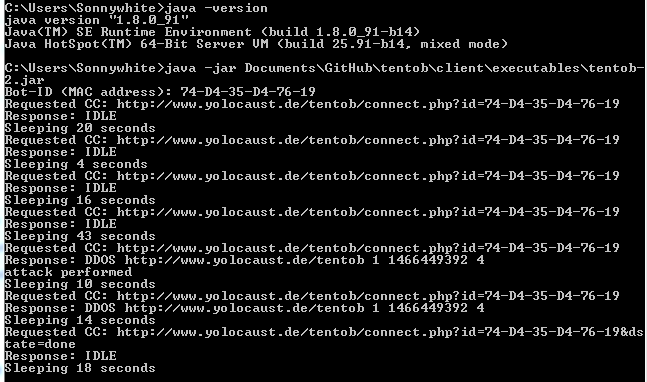
\includegraphics[scale=0.6]{showcase-client.png}
	}
	
	\frame{
		\frametitle{Build Your Own Botnet - \texttt{tentoB}}
		\framesubtitle{Verbesserungen bzw. fehlende Features}
		\begin{itemize}[<+->]
			\item siehe Adminbereich
			\item mehrere "`Kunden"'-Accounts f�r Admin-Bereich (Zuteilung Bots)
			\item verschl�sselte Kommunikation
			\item abgestimmter Zeitpunkt f�r DDoS (Uhrzeit, Zeitzone)
			\item variable URL f�r DDoS-Attacke
			\item {\color{red}Einschleusen der Client-Anwendung}
			\item {\color{red}Client-Anwendung verbergen}
			\item {\color{red}Server verbergen, mehr Server aufstellen}
			\item {\color{red}Provider und Host finden}
		\end{itemize}
	}
	
	\addtocounter{framenumber}{-2}
	
  {
		\setbeamertemplate{footline}{}
		\frame{\center{\Large{Fragen?}}}
		
		\frame{\center{\Large{Vielen Dank f�r Ihre Aufmerksamkeit!}}}
	}

\end{document}